\chapter{Mathematical Background}
\label{chap:数学的知識}

\section{Notation}

In this book, we primarily deal with real numbers.
Unless otherwise specified, all numbers are assumed to be real.
The notation is as follows: a scalar is denoted by $a \in \mathbb{R}$, an $N$-dimensional vector by ${\bf a} \in \mathbb{R}^{N}$, and an $N \times M$ matrix by $A \in \mathbb{R}^{N \times M}$.
We also frequently use the identity matrix.
To make the dimension explicit, we attach a subscript; for example, the $N$-dimensional identity matrix is denoted by $I_{N}$.














\section{Jacobian}

In this book, we primarily make use of {\bf optimization}.
Optimization refers to the process of minimizing (or maximizing) a function $f({\bf x})$ defined over a variable ${\bf x} = \left( x_{1}, \cdots, x_{N} \right)^{\top} \in \mathbb{R}^{N}$.
Such a function is often referred to as a cost function in the context of optimization.
The goal is to determine the variable ${\bf x}$ that minimizes (or maximizes) the value of $f$.
There exist various approaches to perform optimization, but a fundamental step is to compute the gradient of the function, which is defined in equation~(\ref{eq:scholar_function_jacobian}).
%
\begin{align}
  \frac{ \partial f({\bf x}) }{ \partial {\bf x} } =
  \left( \begin{matrix}
    \frac{ \partial f({\bf x}) }{ \partial x_{1} } &
    \cdots                                         &
    \frac{ \partial f({\bf x}) }{ \partial x_{N} }
  \end{matrix} \right).
  \label{eq:scholar_function_jacobian}
\end{align}
%
The derivative of a function with respect to its vector argument is referred to as the {\bf Jacobian}.
For a vector-valued function ${\bf f}({\bf x}) = \left( f_{1}({\bf x}), \ldots, f_{M}({\bf x}) \right)^{\top} \in \mathbb{R}^{M}$, the Jacobian can also be defined, as expressed in equation~(\ref{eq:vector_function_jacobian}).
%
\begin{align}
  \frac{ \partial {\bf f} \left( {\bf x} \right) }{ \partial {\bf x} } =
  \left( \begin{matrix}
    \frac{ \partial f_{1} \left( {\bf x} \right) }{ \partial x_{1} } &
    \cdots                                             &
    \frac{ \partial f_{1} \left( {\bf x} \right) }{ \partial x_{N} } \\
    %
    \vdots                                             &
    \ddots                                             &
    \vdots                                             \\
    %
    \frac{ \partial f_{M} \left( {\bf x} \right) }{ \partial x_{1} } &
    \cdots                                             &
    \frac{ \partial f_{M} \left( {\bf x} \right) }{ \partial x_{N} } \\
  \end{matrix} \right).
  \label{eq:vector_function_jacobian}
\end{align}
%
In this book, the Jacobian is denoted by $J$, unless otherwise specified.

The computation of the Jacobian is generally carried out according to the definitions given in equations~(\ref{eq:scholar_function_jacobian}) and~(\ref{eq:vector_function_jacobian}).
However, it can also be derived in a slightly different manner, and in this book we primarily adopt this approach.
Specifically, we approximate the change in the function $f({\bf x})$ resulting from a perturbation $\delta {\bf x}$ using a Taylor expansion.
%
\begin{align}
  f \left( {\bf x} + \delta {\bf x} \right) \simeq
  f \left( {\bf x} \right) + 
  J \delta {\bf x} + 
  \frac{1}{2} \delta {\bf x}^{\top} H \delta {\bf x},
  \label{eq:taylor_expansion_approximation_2nd_order}
\end{align}
%
where $H = \partial^{2} f({\bf x}) / \partial {\bf x}^{2}$, which is referred to as the {\bf Hessian}.
By neglecting the second-order infinitesimal terms and assuming that both sides of equation~(\ref{eq:taylor_expansion_approximation_2nd_order}) are equal, we obtain the following expression.
%
\begin{align}
  f \left( {\bf x} + \delta {\bf x} \right) - f \left( {\bf x} \right) = J \delta {\bf x}
  \label{eq:jacobian_difference}
\end{align}
%
In other words, if the difference between $f({\bf x} + \delta {\bf x})$ and $f({\bf x})$ can be expressed in the form $J \delta {\bf x}$, then the Jacobian can be obtained.

As a simple example, consider $f(x) = x^{2}$.
The Jacobian\footnote{Strictly speaking, since the argument is a scalar, it is usually referred to as the derivative; however, in the one-dimensional case, it can formally be regarded as a Jacobian.} of this function is $\partial x^{2} / \partial x = 2x$.
Nevertheless, let us derive the Jacobian using the method shown in equation~(\ref{eq:jacobian_difference}).
%
\begin{align}
  \begin{split}
    (x + \delta x)^{2} - x^{2}
    = & x^{2} + 2 x \delta x + \delta x^{2} - x^{2}, \\
    = & 2 x \delta x,
  \end{split}
  \label{eq:jacobian_difference_example}
\end{align}
%
where the second-order infinitesimal term was neglected by assuming $\delta x^{2} \simeq 0$.
As shown in equation~(\ref{eq:jacobian_difference_example}), we correctly obtained the Jacobian of $f(x) = x^{2}$.
Using this approach, the Jacobian can be computed without directly differentiating the function\footnote{The Jacobian obtained here is derived as a first-order approximation by applying a Taylor expansion and neglecting higher-order infinitesimal terms. In the limit as $\delta x \to 0$, it coincides with the theoretical derivative, whereas for finite differences it provides a numerical approximation.}.













\section{Gauss-Newton Method}
\label{subsec:gauss-newton_method}

The problems addressed in this book are often reduced to optimization problems.
While there exist various methods for solving such problems, in this book we primarily employ the {\bf Gauss-Newton method}.

To introduce the Gauss-Newton method, we first define the state variable ${\bf x} \in \mathbb{R}^{N}$ and the residual (or residual vector) ${\bf r}({\bf x}) \in \mathbb{R}^{M}$, which depends on this state.
Using multiple residual vectors, we then define the following cost function.
%
\begin{align}
  E \left( {\bf x} \right) = \sum_{i} \| {\bf r}_{i} \left( {\bf x} \right) \|_{2}^{2} \in \mathbb{R},
\end{align}
%
where $\| \cdot \|_{2}^{2}$ denotes the squared Euclidean norm of a vector.
The state that minimizes the cost function is then defined as follows.
%
\begin{align}
  {\bf x}^{*} = \argmin_{ {\bf x} } E \left( {\bf x} \right).
\end{align}
%
This means that we seek a state ${\bf x}^{*}$ within the domain of ${\bf x}$ that minimizes the cost function $E({\bf x})$.
Such a solution is referred to as the {\bf optimal solution}.

To consider optimization using the Gauss-Newton method, we first approximate the residual vector by a first-order Taylor expansion.
%
\begin{align}
  {\bf r} \left( {\bf x} + \delta {\bf x} \right) \simeq {\bf r} \left( {\bf x} \right) + J \delta {\bf x},
  \label{eq:error_vector_taylor}
\end{align}
%
where $J$ denotes the Jacobian of the residual vector ${\bf r}$ with respect to the state vector ${\bf x}$, i.e., $J = \partial {\bf r} / \partial {\bf x} \in \mathbb{R}^{M \times N}$.
Next, we consider the squared norm of the approximated residual vector given in equation~(\ref{eq:error_vector_taylor}).
%
\begin{align}
  \begin{split}
    \left( {\bf r} + J \delta {\bf x} \right)^{\top} \left( {\bf r} + J \delta {\bf x} \right)
    %
    = & \left( {\bf r}^{\top} + \delta {\bf x}^{\top} J^{\top} \right) \left( {\bf r} + J \delta {\bf x} \right), \\
    %
    = & {\bf r}^{\top} {\bf r} + {\bf r}^{\top} J \delta {\bf x} + \delta {\bf x}^{\top} J^{\top} {\bf r} + \delta {\bf x}^{\top} J^{\top} J \delta {\bf x}, \\
    %
    = & {\bf r}^{\top} {\bf r} + 2 \delta {\bf x}^{\top} J^{\top} {\bf r} + \delta {\bf x}^{\top} J^{\top} J \delta {\bf x},
  \end{split}
  \label{eq:error_vector_taylor_sq_norm}
\end{align}
%
where we use the relation ${\bf r}^{\top} J \delta {\bf x} = \delta {\bf x}^{\top} J^{\top} {\bf r}$.

Next, we regard equation~(\ref{eq:error_vector_taylor_sq_norm}) as a function of $\delta {\bf x}$, denoted by $f(\delta {\bf x})$, and take its derivative with respect to $\delta {\bf x}$.
%
\begin{align}
  \frac{ \partial f \left( \delta {\bf x} \right) }{ \partial \delta {\bf x} } = 2 J^{\top} {\bf r} + 2 J^{\top} J \delta {\bf x}.
  \label{eq:error_vector_taylor_sq_norm_partial}
\end{align}
%
Then, by assuming that equation~(\ref{eq:error_vector_taylor_sq_norm_partial}) equals ${\bf 0}$, the following expression holds.
%
\begin{align}
  J^{\top} J \delta {\bf x} = -J^{\top} {\bf r}.
  \label{eq:gauss_newton_update_value}
\end{align}

Here, let us consider $\delta {\bf x}$ that satisfies equation~(\ref{eq:gauss_newton_update_value}).
The function $f(\delta {\bf x})$ represents an approximation of the residual vector when the state is perturbed by $\delta {\bf x}$, and its squared norm is computed.
By differentiating this with respect to $\delta {\bf x}$ and setting the result equal to ${\bf 0}$, we can obtain the value of $\delta {\bf x}$ that minimizes the squared norm of the approximated residual vector.
In other words, updating ${\bf x}$ by this $\delta {\bf x}$ decreases the cost function.

In the derivation of equation~(\ref{eq:error_vector_taylor_sq_norm}), we considered the approximation of a single residual vector.
However, the actual cost function involves the sum of squared norms of multiple residual vectors.
Therefore, it is necessary to approximate the cost function when the state ${\bf x}$ is perturbed by $\delta {\bf x}$, which leads to equation~(\ref{eq:cost_function_taylor}).
%
\begin{align}
  E \left( {\bf x} + \delta {\bf x} \right) \simeq \sum_{i} \left( {\bf r}_{i}^{\top} {\bf r}_{i} + 2 \delta {\bf x}^{\top} J_{i}^{\top} {\bf r}_{i} + \delta {\bf x}^{\top} J_{i}^{\top} J_{i} \delta {\bf x} \right).
  \label{eq:cost_function_taylor}
\end{align}
%
Similarly, by differentiating equation~(\ref{eq:cost_function_taylor}) with respect to $\delta {\bf x}$ and setting the result to ${\bf 0}$, we obtain the following expression.
%
\begin{align}
  \sum_{i} J_{i}^{\top} J_{i} \delta {\bf x} = -\sum_{i} J_{i}^{\top} {\bf r}_{i}.
  \label{eq:gauss_newton_update_sum}
\end{align}
%
Here, for simplicity, we introduce the following variables.
%
\begin{align}
  \begin{gathered}
    H = \sum_{i} J_{i}^{\top} J_{i}, \\
    {\bf b} = \sum_{i} J_{i}^{\top} {\bf r}_{i}.
  \end{gathered}
  \label{eq:hessian_and_gradient_gauss_newton}
\end{align}
%
With this notation, equation~(\ref{eq:gauss_newton_update_sum}) can be written as $H \delta {\bf x} = -{\bf b}$.
Here, $H$ and ${\bf b}$ are often referred to as the Hessian and the gradient, respectively.
In optimization using the Gauss-Newton method, once $\delta {\bf x}$ satisfying $H \delta {\bf x} = -{\bf b}$ is obtained, the state is updated as follows.
%
\begin{align}
  {\bf x} \leftarrow {\bf x} + \delta {\bf x}.
  \label{eq:gauss_newton_update_vector}
\end{align}
%
Note that from $H \delta {\bf x} = -{\bf b}$, one can naturally derive $\delta {\bf x} = -H^{-1} {\bf b}$.
However, since $H \in \mathbb{R}^{N \times N}$, the direct computation of the inverse becomes intractable when $N$ is large.
For this reason, it is uncommon to compute the inverse explicitly, and we instead refer to $\delta {\bf x}$ as ``the solution satisfying $H \delta {\bf x} = -{\bf b}$.''
When $N$ is not large, computing $H^{-1}$ directly does not pose a practical problem.









\section{Robust Kernel}

In performing optimization, multiple residual vectors are defined.
However, if incorrect correspondences (i.e., mismatches) are used to construct residual vectors, they can adversely affect the optimization.
Typically, the norm of residual vectors arising from mismatches tends to be larger than that of residuals from correct correspondences.
Therefore, it is effective to suppress the influence on optimization according to the magnitude of the residual norm.
To achieve this effect, a {\bf robust kernel} can be introduced.

In general, a cost function with a robust kernel is expressed as follows.
%
\begin{align}
  E \left( {\bf x} \right) = \sum_{i} \rho \left( \| {\bf r}_{i} \left( {\bf x} \right) \|_{2}^{2} \right),
  \label{eq:cost_function_robust_kernel}
\end{align}
%
where $\rho(\cdot)$ represents the robust kernel.
Various types of robust kernels exist, but in this book we employ the {\bf Huber loss}.
The Huber loss is defined as follows.
%
\begin{align}
  \rho \left( s \right)
  =
  \begin{cases}
    s                                & {\rm if} ~ s \leq \delta^{2} \\
    2 \delta \sqrt{ s } - \delta^{2} & {\rm otherwise}
  \end{cases},
  \label{eq:huber_loss}
\end{align}
%
where $\delta$ is an arbitrary positive real number.

To consider the Gauss-Newton method with the Huber loss, we evaluate the Huber loss applied to the linear approximation of the residual vector, as shown in equation~(\ref{eq:error_vector_taylor_sq_norm}); that is, ${\bf r}({\bf x} + \delta {\bf x})$ is approximated by ${\bf r}({\bf x}) + J \delta {\bf x}$.
%
\begin{align}
  \rho \left( \left( {\bf r} + J \delta {\bf x} \right)^{\top} \left( {\bf r} + J \delta {\bf x} \right) \right)
  =
  \rho \left( {\bf r}^{\top} {\bf r} + 2 \delta {\bf x}^{\top} J^{\top} {\bf r} + \delta {\bf x}^{\top} J^{\top} J \delta {\bf x} \right).
\end{align}
%
Here, let $s = {\bf r}^{\top} {\bf r} + 2 \delta {\bf x}^{\top} J^{\top} {\bf r} + \delta {\bf x}^{\top} J^{\top} J \delta {\bf x}$.
From equation~(\ref{eq:huber_loss}), when $s \leq \delta^{2}$, the value of $s$ is directly used.
Therefore, we focus on the case where $s$ exceeds $\delta^{2}$, and differentiate the result of substituting the given $s$ into the Huber loss with respect to $\delta {\bf x}$.
%
\begin{align}
  \begin{split}
    \frac{ \partial \rho \left( s \right) }{ \partial \delta {\bf x} }
    = &
    \frac{ \partial \rho \left( s \right) }{ \partial s }
    \frac{ \partial s }{ \partial \delta {\bf x} }, \\
    = &
    \frac{ \delta }{ \sqrt{s} } \left( 2 J^{T} {\bf r} + 2 J^{\top} J \delta {\bf x} \right).
  \end{split}
  \label{eq:huber_loss_diff}
\end{align}
%
Then, by assuming that equation~(\ref{eq:huber_loss_diff}) equals ${\bf 0}$, we obtain the following result.
%
\begin{align}
  \frac{ \delta }{ \sqrt{s} } J^{\top} J \delta {\bf x} = -\frac{ \delta }{ \sqrt{s} } J^{T} {\bf r}.
  \label{eq:gauss_newton_update_value_huber_loss}
\end{align}
%
Compared with equation~(\ref{eq:gauss_newton_update_value}), equation~(\ref{eq:gauss_newton_update_value_huber_loss}) contains the factor $\delta / \sqrt{s}$ on both sides.
Note that this factor can, in principle, be eliminated.
However, since in practice we consider the sum of multiple residual vectors, and the value of $\delta / \sqrt{s}$ differs for each residual vector, we retain it in the formulation.

Then, as shown in equation~(\ref{eq:hessian_and_gradient_gauss_newton}), by defining the Hessian and the gradient while taking all residual vectors into account, we obtain the following.
%
\begin{align}
  \begin{gathered}
    H = \sum_{i} \rho^{\prime} \left( s_{i} \right) J_{i}^{\top} J_{i}, \\
    {\bf b} = \sum_{i} \rho^{\prime} \left( s_{i} \right) J_{i}^{\top} {\bf r}_{i},
  \end{gathered}
  \label{eq:hessian_and_gradient_gauss_newton_huber_loss}
\end{align}
%
where $\rho^{\prime}(s) = \partial \rho(s) / \partial s$, which, from equation~(\ref{eq:huber_loss}), is given as follows.
%
\begin{align}
  \rho^{\prime} \left( s \right)
  =
  \begin{cases}
    1                             & {\rm if} ~ s \leq \delta^{2} \\
    \frac{ \delta }{ \sqrt{ s } } & {\rm otherwise}
  \end{cases}.
  \label{eq:huber_loss_prime}
\end{align}
%

However, since $s = {\bf r}^{\top} {\bf r} + 2 \delta {\bf x}^{\top} J^{\top} {\bf r} + \delta {\bf x}^{\top} J^{\top} J \delta {\bf x}$, $\rho^{\prime}(\cdot)$ directly depends on $\delta {\bf x}$.
As a result, the linear structure of the Gauss-Newton method breaks down, and the update cannot be obtained in the form shown in equation~(\ref{eq:gauss_newton_update_sum}).
To address this, we let $s_{0} = {\bf r}^{\top} {\bf r}$ and $\delta s = 2 \delta {\bf x}^{\top} J^{\top} {\bf r} + \delta {\bf x}^{\top} J^{\top} J \delta {\bf x}$, and approximate $\rho^{\prime}(s) \simeq \rho^{\prime}(s_{0}) + \rho^{\prime \prime}(s_{0}) \delta s$.
Then, by regarding $\rho^{\prime \prime}(s_{0}) \delta s$ as a higher-order infinitesimal term and neglecting it, we approximate $\rho^{\prime}(s) \simeq \rho^{\prime}(s_{0})$.
Consequently, $\rho^{\prime}(s) \simeq \rho^{\prime}(s_{0})$ no longer depends on $\delta {\bf x}$, thereby preserving the linear structure of the Gauss-Newton method.

Finally, we define the weight $w = \rho^{\prime}({\bf r}^{\top} {\bf r})$ and specify the Hessian and gradient as follows.
%
\begin{align}
  \begin{gathered}
    H = \sum_{i} w_{i} J_{i}^{\top} J_{i}, \\
    {\bf b} = \sum_{i} w_{i} J_{i}^{\top} {\bf r}_{i}.
  \end{gathered}
  \label{eq:hessian_and_gradient_gauss_newton_huber_loss_weight}
\end{align}
%
By using these $H$ and ${\bf b}$ to solve for $\delta {\bf x}$ satisfying $H \delta {\bf x} = -{\bf b}$, and updating the state according to equation~(\ref{eq:gauss_newton_update_vector}), optimization with the Gauss-Newton method incorporating the Huber loss can be performed.
Although the derivation of the state update for the Gauss-Newton method with the Huber loss is somewhat more involved, the actual implementation is straightforward: it simply requires computing the function given in equation~(\ref{eq:huber_loss_prime}) as a weight and applying it to the corresponding Hessian and gradient.
In many cases, employing the Huber loss makes the optimization more robust.
















\section{Lie Group and Lie Algebra}

In this book, we frequently make use of {\bf Lie groups} and {\bf Lie algebras}.
While a rigorous explanation of Lie groups and Lie algebras is beyond the scope of this text, throughout this book the term Lie group will specifically refer to {\bf rotation matrices} and {\bf rigid transformation matrices}.

A rotation matrix is defined as follows.
%
\begin{align}
  \{R \in \mathbb{R}^{3 \times 3} | R^{\top} R = I, {\rm det}(R) = 1\}.
  \label{eq:def_SO3}
\end{align}
%
A rotation matrix, also referred to as the Special Orthogonal group in three dimensions (${\rm SO}(3)$), represents rotations in three-dimensional space.
A rigid transformation matrix is defined as follows.
%
\begin{align}
  \left\{ \left( \begin{matrix} R & {\bf t} \\ {\bf 0}^{\top} & 1 \end{matrix} \right) \in \mathbb{R}^{4 \times 4} | R \in {\rm SO}(3), {\bf t} \in \mathbb{R}^{3} \right\}.
  \label{eq:def_SE3}
\end{align}
%
A rigid transformation matrix, also referred to as the Special Euclidean group in three dimensions (${\rm SE}(3)$), represents a pose in three-dimensional space, consisting of both rotation and translation.
In LIO and SLAM, the state is typically represented using ${\rm SO}(3)$ and ${\rm SE}(3)$.
As is evident from equation~(\ref{eq:def_SE3}), the variables that constitute $T$ are ${\bf t}$ and $R$.
Therefore, in this book we often adopt the simplified notation $T = \left( R \mid {\bf t} \right)$.

The advantage of using Lie groups is that rotations can be handled smoothly and in a mathematically natural way, without sudden jumps or discontinuities in their representation.
Although the details are omitted here, such spaces are referred to as {\bf manifolds}.
While the concept may feel somewhat abstract at first, let us consider the simple example of planar rotation, namely an angle $\theta$ in the $xy$-plane.
The angle $\theta$ is usually defined in the range $0 \leq \theta < 2\pi$ (or $-\pi \leq \theta < \pi$).
Although $\theta = 0$ and $\theta = 2\pi$ are numerically different, they represent the same rotational state.
Consequently, using $\theta$ directly as a representation may give the appearance of discontinuity. 
By contrast, Lie groups allow changes in rotation to be represented on a ``seamless space,'' enabling continuous treatment from start to finish.
Moreover, operations such as addition and differentiation can be performed under a unified mathematical framework, ensuring consistency and smoothness.

On the other hand, representing states on Lie groups makes the treatment somewhat less intuitive.
For example, suppose the robot state is represented by a vector ${\bf x}$ in some vector space.
If the robot state changes by $\Delta {\bf x}$, one might intuitively expect the new state to be given by the simple addition ${\bf x} + \Delta {\bf x}$ (noting that, as mentioned earlier, special care must be taken when angles such as $\theta$ are involved due to their defined ranges).
However, as shown in equations~(\ref{eq:def_SO3}) and~(\ref{eq:def_SE3}), ${\rm SO}(3)$ and ${\rm SE}(3)$ are subject to specific constraints, and performing such addition would violate these constraints.

For instance, let the change in pose, including both translation and rotation in three-dimensional space, be defined as $\Delta T \in {\rm SE}(3)$ as follows.
%
\begin{align}
  \Delta T
%
  = \left( \begin{matrix}
      \Delta R       & \Delta {\bf t} \\
      {\bf 0}^{\top} & 1
    \end{matrix} \right).
\end{align}
%
If we consider the simple addition of $T$ and $\Delta T$, it can be written as follows.
%
\begin{align}
  T + \Delta T
%
  = \left( \begin{matrix}
      R + \Delta R       & {\bf t} + \Delta {\bf t} \\
      {\bf 0}^{\top}     & 2
    \end{matrix} \right) \notin {\rm SE}(3).
\end{align}
%
It is clear that $T + \Delta T$ does not satisfy equation~(\ref{eq:def_SE3}), and therefore it does not represent a rigid transformation matrix.
To reflect the change while preserving the constraints of ${\rm SE}(3)$, we compute $T \Delta T$\footnote{Since the result of matrix multiplication depends on whether it is applied from the left or the right, the choice of how $\Delta T$ acts is important. In this book, changes associated with motion are generally modeled using right multiplication.}.
%
\begin{align}
  T \Delta T
%
  = \left( \begin{matrix}
      R \Delta R     & R \Delta {\bf t} + {\bf t} \\
      {\bf 0}^{\top} & 1
    \end{matrix} \right) \in {\rm SE}(3).
  \label{eq:se3_add}
\end{align}
%
Moreover, when the difference between $T_{1}, T_{2} \in {\rm SE}(3)$ is denoted as $\Delta T$, the relation $T_{1} \Delta T = T_{2}$ holds.
Thus, the difference between $T_{1}$ and $T_{2}$ is defined as follows.
%
\begin{align}
  \begin{split}
    \Delta T
%
    & = T_{1}^{-1} T_{2}, \\
%
    & = \left( \begin{matrix}
          R_{1}^{\top} R_{2} & R_{2} ({\bf t}_{2} - {\bf t}_{1}) \\
          {\bf 0}^{\top}     & 1
        \end{matrix} \right) \in {\rm SE}(3).
  \end{split}
  \label{eq:se3_diff}
\end{align}

By using equations~(\ref{eq:se3_add}) and~(\ref{eq:se3_diff}), state changes in the space of ${\rm SE}(3)$ (or ${\rm SO}(3)$) can be expressed.
However, compared to addition and subtraction in vector spaces, these operations are less intuitive and are not in a form to which the Gauss-Newton method, as described in the previous sections, can be directly applied.
To address this, we consider whether states represented on Lie groups can be associated with vectors.
This is made possible by employing the Lie algebra, which is the vector space corresponding to a Lie group.
Specifically, the Lie algebras associated with ${\rm SO}(3)$ and ${\rm SE}(3)$ are denoted by $\mathfrak{so}(3)$ and $\mathfrak{se}(3)$, respectively.
Strictly speaking, $\mathfrak{so}(3)$ and $\mathfrak{se}(3)$ are sets of matrices in $\mathbb{R}^{3 \times 3}$ and $\mathbb{R}^{4 \times 4}$, but since they can be parameterized by three and six independent real numbers, respectively, they can be represented as three- and six-dimensional vectors.
Furthermore, the mappings between ${\rm SO}(3)$ and $\mathfrak{so}(3)$, and between ${\rm SE}(3)$ and $\mathfrak{se}(3)$, are referred to as the {\bf exponential map} and the {\bf logarithm map}, respectively.
%
\begin{align}
  \begin{gathered}
    \exp: \mathfrak{so}(3) \rightarrow {\rm SO}(3), \\
    \log: {\rm SO}(3) \rightarrow \mathfrak{so}(3), \\
  \end{gathered}
  \label{eq:so3_exp_log_maps}
\end{align}
%
\begin{align}
  \begin{gathered}
    \exp: \mathfrak{se}(3) \rightarrow {\rm SO}(3), \\
    \log: {\rm SO}(3) \rightarrow \mathfrak{se}(3). \\
  \end{gathered}
  \label{eq:se3_exp_log_maps}
\end{align}
%
Note that the exponential and logarithm maps shown in equations~(\ref{eq:so3_exp_log_maps}) and~(\ref{eq:se3_exp_log_maps}) are distinct.
However, in this book we do not explicitly specify whether ${\rm SO}(3)$ or ${\rm SE}(3)$ is used in each case; instead, the type of map is inferred from the variable provided as the argument.

By employing Lie algebras, optimization methods such as the Gauss-Newton method can be applied even when the states are represented on Lie groups.
Before discussing optimization using Lie algebras, however, we first provide an explanation of the exponential and logarithm maps.
The derivations of these maps are omitted, and only their computational procedures are presented.













\subsection{Exponential and Logarithm Maps}

For a three-dimensional vector $\boldsymbol{\phi}$, the exponential map shown in equation~(\ref{eq:so3_exp_log_maps}) is defined as follows.
%
\begin{align}
  \begin{gathered}
    \theta = \| \boldsymbol \phi \|_{2}, \\
    %
    \exp \left( \boldsymbol \phi^{^\wedge} \right)
    =
    I_{3} +
    \frac{ \sin \theta }{ \theta } \boldsymbol \phi{^\wedge} +
    \frac{ 1 - \cos \theta }{ \theta^{2} } \left( \boldsymbol \phi{^\wedge} \right)^{2},
  \end{gathered}
  \label{eq:so3_exp_map}
\end{align}
%
where $\left( \cdot \right)^{\wedge}$ denotes the operation that maps a three-dimensional vector to $\mathfrak{so}(3)$ (or a six-dimensional vector to $\mathfrak{se}(3)$).
In the case of a three-dimensional vector, it can also be regarded as the operation that generates a {\bf skew-symmetric matrix}.
%
\begin{align}
  \boldsymbol \phi^{^\wedge}
%
  = \left( \begin{matrix}
      0         & -\phi_{z} & \phi_{y} \\
      \phi_{z}  & 0         & -\phi_{x} \\
      -\phi_{y} & \phi_{x}  & 0
    \end{matrix} \right) \in \mathfrak{so}(3),
  \label{eq:skew_symmetric_matrix}
\end{align}
%
As a brief aside, one property of skew-symmetric matrices is that ${\bf a}^{\wedge} {\bf b} = -{\bf b}^{\wedge} {\bf a}$, where ${\bf a}, {\bf b} \in \mathbb{R}^{3}$.
%
\begin{align}
  \begin{split}
    {\bf a}^{^\wedge} {\bf b}
%
    & = \left( \begin{matrix}
          -a_{z} b_{y} + a_{y} b_{z} \\
           a_{z} b_{x} - a_{x} b_{z} \\
          -a_{y} b_{x} + a_{x} b_{y}
        \end{matrix} \right), \\
%
    & = \left( \begin{matrix}
          0      &  b_{z} & -b_{y} \\
          -b_{z} & 0      & b_{x} \\
          b_{y}  & -b_{x} & 0
        \end{matrix} \right),
        \left( \begin{matrix}
          a_{x} \\
          a_{y} \\
          a_{z}
        \end{matrix} \right) \\
%
     & = -{\bf b}^{\wedge} {\bf a}.
  \end{split}
\end{align}
%
This property will be used later when computing Jacobians in the implementation.

Furthermore, the logarithm map shown in equation~(\ref{eq:so3_exp_log_maps}) is defined as follows.
%
\begin{align}
  \begin{gathered}
    \theta = \arccos \left( \frac{{\rm tr}(R) - 1}{ 2 } \right), \\
    %
    \log( R ) = \frac{ \theta }{ 2 \sin \theta } \left( R - R^{\top} \right).
  \end{gathered}
  \label{eq:so3_log_map}
\end{align}
%
Note that since $\log(R) = \boldsymbol{\phi}^{\wedge} \in \mathfrak{so}(3)$, we define the operation of extracting the three-dimensional vector $\boldsymbol{\phi} = \left( \phi_{x} ~ \phi_{y} ~ \phi_{z} \right)^{\top}$ from this skew-symmetric matrix as follows.
%
\begin{align}
  \boldsymbol \phi = \left( \boldsymbol \phi^{\wedge} \right)^{\vee}.
\end{align}
%
As will be shown later, the operation of extracting a six-dimensional vector from $\mathfrak{se}(3)$ is similarly denoted by $\left( \cdot \right)^{\vee}$.

In equations~(\ref{eq:so3_exp_map}) and~(\ref{eq:so3_log_map}), the parameter $\theta$ appears in the denominator, which makes the computation unstable when $\theta \ll 1$.
Therefore, in the case of $\theta \ll 1$, the computation is approximated as follows.
%
\begin{align}
  \begin{gathered}
    \exp \left( \boldsymbol \phi^{\wedge} \right) \simeq I_{3} + \boldsymbol \phi^{\wedge} + \frac{1}{2} \left( \boldsymbol \phi^{\wedge} \right)^{2}, \\
%
    \log \left( R \right) \simeq \frac{1}{2} \left( R - R^{\top} \right).
  \end{gathered}
  \label{eq:so3_exp_log_maps_approx}
\end{align}
%

Next, in order to consider the exponential and logarithm maps for ${\rm SE}(3)$, we define the six-dimensional vector $\boldsymbol{\xi} = \left( {\bf v}^{\top} ~ \boldsymbol{\phi}^{\top} \right)^{\top}$.
We then define the operation that maps this six-dimensional vector to $\mathfrak{se}(3)$ as follows\footnote{In equation~(\ref{eq:skew_symmetric_matrix}), $\left( \cdot \right)^{\wedge}$ is defined as the operation that generates a skew-symmetric matrix corresponding to a three-dimensional vector. In the case of a six-dimensional vector, however, it is treated as the operation that generates an element of $\mathfrak{se}(3)$, as shown in equation~(\ref{eq:se3_wedge}).}.
%
\begin{align}
  \boldsymbol \xi^{\wedge} = \left( \begin{matrix}
    \boldsymbol \phi^{\wedge} & {\bf v} \\
    {\bf 0}^{\top}            & 0
  \end{matrix} \right) \in \mathfrak{se}(3),
  \label{eq:se3_wedge}
\end{align}
%
where $\boldsymbol{\phi}^{\wedge}$ denotes the operation that returns the skew-symmetric matrix defined in equation~(\ref{eq:skew_symmetric_matrix}).
Using equation~(\ref{eq:se3_wedge}), the exponential map shown in equation~(\ref{eq:se3_exp_log_maps}) is defined as follows.
%
\begin{align}
  \exp \left( \boldsymbol \xi^{\wedge} \right) = \left( \begin{matrix}
    \exp \left( \boldsymbol \phi^{\wedge} \right) & J_{l} \left( \boldsymbol \phi^{\wedge} \right) {\bf v} \\
    {\bf 0}^{\top}                                & 1
  \end{matrix} \right),
  \label{eq:se3_exp_map}
\end{align}
%
where $\exp\left( \boldsymbol{\phi}^{\wedge} \right)$ corresponds to the expression given in equation~(\ref{eq:so3_exp_map}), and $J_{l}(\cdot)$ denotes the left Jacobian, which is defined as follows.
%
\begin{align}
  J_{l} \left( \boldsymbol \phi^{\wedge} \right)
  =
  I_{3} +
  \frac{ 1 - \cos \theta }{ \theta^{2} } \boldsymbol \phi^{\wedge} +
  \frac{ \theta - \sin \theta }{ \theta^{3} } \left( \boldsymbol \phi^{\wedge} \right)^{2},
  \label{eq:so3_left_jacobian}
\end{align}
%
where $\theta = \| \boldsymbol{\phi} \|_{2}$.

The logarithm map shown in equation~(\ref{eq:se3_exp_log_maps}) is defined as follows.
%
\begin{align}
  \log \left( T \right) = \left( \begin{matrix}
    \boldsymbol \phi^{\wedge} & J_{l}^{-1} \left( \boldsymbol \phi \right) {\bf t} \\
    {\bf 0}^{\top}            & 0
  \end{matrix} \right),
  \label{eq:se3_log_map}
\end{align}
%
where $J_{l}^{-1}(\cdot)$ denotes the inverse of the left Jacobian, which is defined as follows.
%
\begin{align}
  J_{l}^{-1} \left( \boldsymbol \phi \right)
  =
  I_{3} -
  \frac{1}{2} \boldsymbol \phi^{\wedge} + 
  \left( \frac{1}{ \theta^{2} } - \frac{ 1 + \cos \theta }{ 2 \theta \sin \theta } \right) \left( \boldsymbol \phi^{\wedge} \right)^{2}.
  \label{eq:so3_left_jacobian_inverse}
\end{align}
%
Similarly, $\theta = \| \boldsymbol{\phi} \|_{2}$.
Note that since $\log(T) \in \mathfrak{se}(3)$ is a matrix in $\mathbb{R}^{4 \times 4}$, we define the operation of extracting the six-dimensional vector $\boldsymbol{\xi}$ from it as follows.
%
\begin{align}
  \begin{split}
    \boldsymbol \xi
%
    = & \left( \begin{matrix}
      J_{l}^{-1} \left( \boldsymbol \phi \right) {\bf t} \\
      \boldsymbol \phi
    \end{matrix} \right), \\
%
    = & \left( \log \left( T \right) \right)^{\vee},
  \end{split}
\end{align}
%
where $\boldsymbol{\phi} = \left( \log(R) \right)^{\vee}$.

Note that in equations~(\ref{eq:so3_left_jacobian}) and~(\ref{eq:so3_left_jacobian_inverse}), the parameter $\theta$ also appears in the denominator.
Therefore, when $\theta \ll 1$, it is necessary to perform approximate computations, as shown in equation~(\ref{eq:so3_exp_log_maps_approx}), in order to avoid numerical instability.











\subsection{State Update via Lie Algebra}

As described above, the logarithm map enables mapping elements of a Lie group to elements of its Lie algebra, thereby allowing optimization to be applied in a vector space.
This makes it possible, for example, to apply nonlinear optimization algorithms such as the Gauss-Newton method to Lie groups.
However, since the final state must be represented as an element of the Lie group, we summarize here the procedure for state update via Lie algebra.
In the following, we focus on ${\rm SE}(3)$, but the same idea can also be applied to ${\rm SO}(3)$.

For instance, suppose that by using the Gauss-Newton method or a similar approach, an update $\delta \boldsymbol{\xi} \in \mathbb{R}^{6}$ on the Lie algebra corresponding to the state $T \in {\rm SE}(3)$ is obtained.
This update is then mapped back to the Lie group via the exponential map, and the actual state update is performed as follows.
%
\begin{align}
  T \leftarrow \exp \left( \delta \boldsymbol \xi^{\wedge} \right) T.
  \label{eq:se3_update_left}
\end{align}
%
This operation can also be regarded as adding the Lie algebra element $\delta \boldsymbol{\xi}$ to the Lie group element $T$, and in correspondence with equation~(\ref{eq:gauss_newton_update_vector}), it is sometimes written as follows.
%
\begin{align}
  T \leftarrow T \boxplus \delta \boldsymbol \xi.
  \label{eq:se3_update_left_boxplus}
\end{align}
%
In equation~(\ref{eq:se3_update_left}), the state is updated by multiplying $\exp \left( \delta \boldsymbol{\xi}^{\wedge} \right)$ from the left.
This is because, when computing the gradient in optimization, we consider the change in the residual with respect to perturbations applied from the left on the Lie group.
If perturbations from the right are considered instead, $\exp \left( \delta \boldsymbol{\xi}^{\wedge} \right)$ must be multiplied from the right, and care must be taken in this case.

Assuming that $\boldsymbol{\xi} = \left( \log(T) \right)^{\vee}$, the updated state vector on the Lie algebra becomes $\boldsymbol{\xi} + \delta \boldsymbol{\xi}$.
If $\delta \boldsymbol{\xi}$ is regarded as an infinitesimal perturbation, the {\bf Baker-Campbell-Hausdorff} (BCH) expansion leads to the following approximation.
%
\begin{align}
  \begin{split}
    \exp\left( (\boldsymbol \xi + \delta \boldsymbol \xi)^{\wedge} \right)
    \simeq & 
    \exp(\delta \boldsymbol \xi^{\wedge}) \exp(\boldsymbol \xi^{\wedge}), \\
    = &
    \exp(\delta \boldsymbol \xi^{\wedge}) T.
  \end{split}
\end{align}
%
Therefore, it can be confirmed that the state update can be performed as shown in equation~(\ref{eq:se3_update_left}).












\subsection{Jacobian Computation Using Lie Groups}

As described in Section~\ref{subsec:gauss-newton_method}, deriving the Jacobian is essential when applying the Gauss-Newton method.
For example, suppose we have a residual vector ${\bf r} \in \mathbb{R}^{N}$ that depends on $T \in {\rm SE}(3)$.
To obtain the Jacobian, it suffices to determine $J$ that satisfies the following equation.
%
\begin{align}
  {\bf r} \left( \exp \left( \delta \boldsymbol \xi^{\wedge} \right) T \right) - {\bf r}(T)
= J \delta \boldsymbol \xi.
\end{align}
%
Note that $J \in \mathbb{R}^{N \times 6}$ (or $\mathbb{R}^{N \times 3}$ in the case of ${\bf r}(R) \in \mathbb{R}^{N}, ; R \in {\rm SO}(3)$).
Examples of defining residual vectors and deriving their Jacobians are presented in the following chapters.

In differentiating residual vectors, it is sometimes necessary to compute derivatives between elements of Lie groups.
To illustrate this, let us first consider the simple case of $\partial T / \partial T$.
In this case, it suffices to determine the Jacobian $J$ that satisfies the following equation.
%
\begin{align}
  T^{-1} \left( \exp \left( \delta \boldsymbol \xi^{\wedge} \right) T \right) = I_{4} + \left( J \delta \boldsymbol \xi \right)^{\wedge}.
  \label{eq:dT_dT}
\end{align}
%
This corresponds to considering the difference between $\exp \left( \delta \boldsymbol{\xi}^{\wedge} \right) T$ and $T$, as shown in equation~(\ref{eq:se3_diff}).
In particular, since $T^{-1} T = I_{4}$, this amounts to analyzing infinitesimal variations around the identity element of the Lie group.
Therefore, this is equivalent to considering the expression $f({\bf x} + \delta {\bf x}) - f({\bf x}) = J \delta {\bf x}$ in a vector space.
Note, however, that $J \delta \boldsymbol{\xi}$ is a six-dimensional vector, and thus it cannot be directly added to $I_{4}$.
Instead, it is mapped to the corresponding element of $\mathfrak{se}(3)$ through the $\left( \cdot \right)^{\wedge}$ operator.
Then, $T^{-1} \exp \left( \delta \boldsymbol{\xi}^{\wedge} \right) T$ can be written as follows.
%
\begin{align}
  T^{-1} \exp \left( \delta \boldsymbol \xi^{\wedge} \right) T = \exp \left( \left( \operatorname{Ad}_{T^{-1}} \delta \boldsymbol \xi \right)^{\wedge} \right),
\end{align}
%
where $\operatorname{Ad}_{T} \in \mathbb{R}^{6 \times 6}$ is referred to as the {\bf adjoint} operator (its detailed definition will be given in the next subsection).
Considering that $\delta \boldsymbol{\xi}$ represents an infinitesimal perturbation, we can approximate it as follows.
%
\begin{align}
  \exp \left( \left( \operatorname{Ad}_{T^{-1}} \delta \boldsymbol \xi \right)^{\wedge} \right) \simeq I_{4} + \left( \operatorname{Ad}_{T^{-1}} \delta \boldsymbol \xi \right)^{\wedge}.
  \label{eq:dT_dT_Ad}
\end{align}
%
By comparing equations~(\ref{eq:dT_dT}) and~(\ref{eq:dT_dT_Ad}), we find that $J = \operatorname{Ad}_{T^{-1}}$, which gives the result of $\partial T / \partial T$.







\subsection{Adjoint}

The adjoint operator is defined as the one that satisfies the following equation.
%
\begin{align}
  \begin{gathered}
    \left( \operatorname{Ad}_{R} \boldsymbol \phi \right)^{\wedge} = R \boldsymbol \phi^{\wedge} R^{\top}, \\
%
    \left( \operatorname{Ad}_{T} \boldsymbol \xi \right)^{\wedge} = T \boldsymbol \xi^{\wedge} T^{-1},
  \end{gathered}
  \label{eq:adjoint}
\end{align}
%
where $\boldsymbol{\phi} \in \mathbb{R}^{3}$ and $\boldsymbol{\xi} \in \mathbb{R}^{6}$.
Although the detailed derivations are omitted, the adjoint operators are defined as follows.
%
\begin{align}
  \operatorname{Ad}_{R} = R,
  \label{eq:adjoint_so3}
\end{align}
%
\begin{align}
  \operatorname{Ad}_{T} = \left( \begin{matrix}
    R & {\bf t}^{\wedge} R \\
    0 & R
  \end{matrix} \right).
  \label{eq:adjoint_se3}
\end{align}







\section{Coordinate Systems and Their Notation}

\begin{figure}[!t]
  \centering
  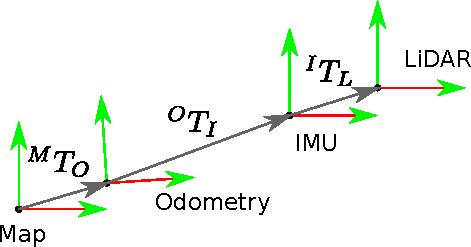
\includegraphics[width=0.4\textwidth]{../figs/frames.pdf}
  \caption{Coordinate frames employed in this work.}
  \label{fig:frames}
\end{figure}

In this book, the coordinate systems considered are primarily the four shown in Fig.~\ref{fig:frames}: the map, odometry, IMU, and LiDAR frames.
Each frame is denoted by the subscripts $M$, $O$, $I$, and $L$, respectively.
For example, when a point ${\bf p}$ is expressed in each of these frames, we place the corresponding superscript in the upper left and denote them as ${}^{M}{\bf p}$, ${}^{O}{\bf p}$, ${}^{I}{\bf p}$, and ${}^{L}{\bf p}$, respectively.
When considering a coordinate transformation (from a Source $S$ to a Target $T$), it is expressed using either of the following notations.
%
\begin{align}
  \begin{gathered}
    {}^{T}{\bf p} = {}^{T}R_{S} {}^{S}{\bf p} + {}^{T}{\bf t}_{S}, \\
%
    {}^{T}{\bf p} = {}^{T}T_{S} {}^{S}{\bf p}.
  \end{gathered}
  \label{eq:point_transformation}
\end{align}
%
Note that when using ${\rm SE}(3)$, we have ${\bf p} \in \mathbb{R}^{4}$, with the fourth element set to $1$.

For example, when transforming a point from the IMU frame to the odometry frame, it is expressed as ${}^{O}{\bf p} = {}^{O}R_{I} {}^{I}{\bf p} + {}^{O}{\bf t}_{I}$, or equivalently as ${}^{O}{\bf p} = {}^{O}T_{I} {}^{I}{\bf p}$.
Similarly, when considering the direct transformation from the IMU frame to the map frame, either of the following notations can be used.
%
\begin{align}
  \begin{gathered}
    {}^{M}{\bf p} = {}^{M}R_{O} \left( {}^{O}R_{I} {}^{I}{\bf p} + {}^{O}{\bf t}_{I} \right) + {}^{M}{\bf t}_{O}, \\
%
    {}^{M}{\bf p} = {}^{M}T_{O} {}^{O}T_{I} {}^{I}{\bf p}.
  \end{gathered}
  \label{eq:point_transformation_synthesis}
\end{align}
%
Here, let ${}^{M}T_{I} = {}^{M}T_{O} {}^{O}T_{I}$, and denote the corresponding translation vector and rotation matrix as ${}^{M}{\bf t}_{I}$ and ${}^{M}R_{I}$, respectively.
With this, equation~(\ref{eq:point_transformation_synthesis}) can be rewritten as a single transformation, as shown in equation~(\ref{eq:point_transformation}).

As for the coordinate transformations illustrated in Fig.~\ref{fig:frames}, in general, the transformation between the IMU and LiDAR, ${}^{I}T_{L}$, is static and thus obtained in advance through calibration.
LIO then estimates ${}^{O}T_{I}$, while SLAM (or localization) estimates ${}^{M}T_{O}$.
However, ${}^{I}T_{L}$ can also be optimized online.
Moreover, in some cases, one may assume that LIO directly estimates the transformation to the map frame, without relying on SLAM or localization.
Therefore, the coordinate relations shown in Fig.~\ref{fig:frames} are not necessarily strict requirements.


